\documentclass{article}
\usepackage[utf8]{inputenc}
\usepackage{kpfonts}
\usepackage{commath}
\usepackage{amsthm}
\usepackage{graphicx}
\usepackage[margin=0.8in]{geometry}

\newcommand{\R}{\ensuremath{\mathbb{R}}}
\newcommand{\N}{\ensuremath{\mathbb{N}}}
\newcommand{\Q}{\ensuremath{\mathbb{Q}}}
\newcommand{\B}{\ensuremath{\mathcal{B}}}
\newcommand{\wrt}{with respect to}
\newcommand{\nbd}{neighborhood}
\newcommand{\Iff}{if and only if}
\newcommand{\ts}{topological space}
\newcommand{\es}{\ensuremath{\emptyset}}
\newcommand{\coleq}{\ensuremath{\coloneqq}}
\newcommand{\powset}[1]{\ensuremath{\mathcal{P}(#1)}}
\newcommand{\define}[1]{\textbf{\underline{#1}}}
\newcommand{\card}[1]{\ensuremath{\mathbf{card} (#1)}}
\newcommand{\func}[3]{\ensuremath{#1: #2 \to #3}}
\newcommand{\closure}[1]{\ensuremath{\overline{#1}}}
\newcommand{\ball}[3]{\ensuremath{B_{#1}^{#2}(#3)}}
\newcommand{\Ball}[3]{\ensuremath{\overline{B}_{#1}^{#2}(#3)}}
\newcommand{\fRR}{\ensuremath{f:\R \to \R}}
\newcommand{\id}{\ensuremath{\mathrm{id}}}
\newcommand{\tp}{\ensuremath{\mathcal{T}}}
\newcommand{\Ts}[2]{\ensuremath{(#1,#2)}}
\newcommand{\tpcof}{\ensuremath{\tp_\text{cof}}}
\newcommand{\tpdisc}{\ensuremath{\tp_\text{disc}}}
\newcommand{\tptriv}{\ensuremath{\tp_\text{triv}}}
\newcommand{\tpeuc}{\ensuremath{\tp_\text{Euc}}}
\newcommand{\Beuc}{\ensuremath{\B_\text{Euc}}}
\newcommand{\union}{\cup}
\newcommand{\Union}{\bigcup}
\newcommand{\inter}{\cap}
\newcommand{\Inter}{\bigcap}
\newcommand{\interior}[1]{\ensuremath{\mathring{#1}}}
\newcommand{\bound}[1]{\ensuremath{\partial #1}}
\renewcommand{\Subset}{\subseteq}
\renewcommand{\Supset}{\supseteq}

\theoremstyle{definition}
\newtheorem*{defn}{Definition}
\newtheorem*{cor}{Corollary}
\newtheorem*{thm}{Theorem}
\newtheorem*{prop}{Proposition}
\newtheorem*{ex}{Ex}
\newtheorem*{lem}{Lemma}

\theoremstyle{remark}
\newtheorem*{rmk}{Remark}

\begin{document}
    \begin{center}
        \textsc{Dillan Marroquin\\MATH 440.1001\\Scribing Week 7\\Due. 15 March 2021\\}
    \end{center}
        
    \noindent\section*{\textbf{\textsc{Lecture 18}}}{
        \subsection*{Homeomorphisms (Continued)}
            \textbf{Q: Which continuous bijections are homeomorphisms?}
            
            \begin{defn}[18.1 Open/Closed maps]
                A map $\func{f}{X}{Y}$ is an \define{open} (or \define{closed} map \Iff{} for each open (or closed) subset $B \Subset X$, the image $f(B) \Subset Y$ is open (or closed).
            \end{defn}
            
            \begin{prop}[18.2]
                Let $\func{f}{X}{Y}$ be a continuous bijection. Then $f$ is a homeomorphism \Iff{} $f$ is an open (or closed) map.
            \end{prop}
            
            \begin{proof}(Only for the Open Case)\\
                ($\implies$) Let $U \Subset X$ be open. Since $\func{f^{-1}}{Y}{X}$ is continuous, $(f^{-1})^{-1}(U)=f(U)$ is open.\\
                ($\impliedby$) Let $\func{f^{-1}}{Y}{X}$ be the set-theoretic inverse to $f$. Let $U \Subset X$ be open. Then $(f^{-1})^{-1}(U)=f(U)$ is open since $f$ is an open map.
            \end{proof}
            
            \begin{ex}[18.3]\hfill
                \begin{enumerate}
                    \item $\func{f}{\R^2}{R}, \, f(x,y) \coleq x$ is an open map.
                    \begin{flushleft}
                        \graphicspath{images}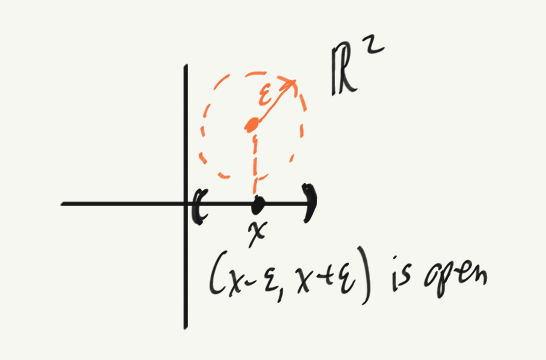
\includegraphics[scale = 0.25]{images/Ex 18.3.png}
                    \end{flushleft}
                        
                    \item $\func{i}{S^2}{\R^3}, \, i(x,y,z)\coleq(x,y,z)$ where $S^2\coleq\{(x,y,z) \in \R^3| x^2+y^2+z^2=1\}$ equipped with the subspace topology is closed.
                \end{enumerate}
            \end{ex}
        
            \begin{prop}[18.4]
                The punctured $n$-sphere is homeomorphic to $\R^n$.
            \end{prop}
            
            \begin{proof}
                Define $\func{f}{S^n-\{\Vec{p}\}}{\R^n}$ via stereographic projection:
                \begin{flushleft}
                    \graphicspath{images}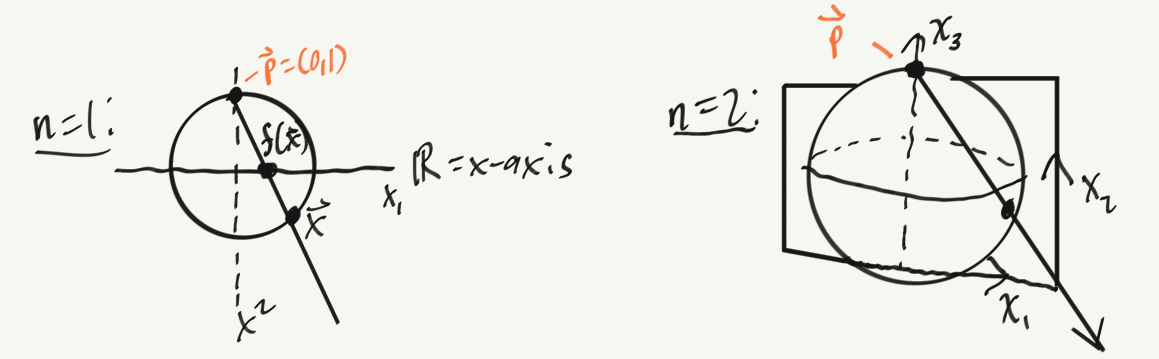
\includegraphics[scale = 0.25]{images/Proof Prop 18.4.png}
                \end{flushleft}
                If $\Vec{x} \in S^n-\{\Vec{p}\}$, let $l$ be the line through $\Vec{x}$ and $\Vec{p}$ in $\R^{n+1}$. Then define $f(\Vec{x}) \coleq$ the intersection of $l$ with the $n$-plane $\{\Vec{x}\in \R^{n+1}|x_{n+1}=0\}=\R^n$. Parameterize $l(t)\coleq (tx_1,tx_2,\ldots,tx_{n+1}-t+1)$ so that $l(0)= \Vec{p}$ and $l(1)=\Vec{x}$.\\
                Solve for $t:$ $tx_{n+1}-t+1=0 \implies t=1/1-x_{n+1}$. Define $f(\Vec{x})\coleq \frac{1}{1-x_{n+1}}(x_1,\ldots,x_n) \in \R^n$. Observe that $f$ is continuous at all $\Vec{x} \in \R^{n+1} \; \forall \Vec{x}$ such that $x_{n+1} \neq 1$.\\
                Cor. 16.4 implies that $f$ is continuous on subspace $S^n-\{\Vec{p}\}$.\\
                Explicitly find an inverse $\func{f^{-1}}{\R^n}{S^n-\{\Vec{p}\}}, \, f^{-1}(\Vec{y})\coleq (r(\Vec{y})y_1,r(\Vec{y})y_2\ldots,r(\Vec{y})y_n, 1-r(\Vec{y})$ where $\Vec{y}=(y_1,\ldots,y_n)$ and $r(\Vec{y})\coleq 2/(1+\norm{\Vec{y}}^2 \neq 0$. This implies that $f^{-1}(\Vec{y})\neq \Vec{p} \; \forall \Vec{y} \in \R^n$. Verify $\norm{f^{-1}(\Vec{y})}^2=1$ so that $f^{-1}(\Vec{y}) \in S^n$.
            \end{proof}
        }
    \noindent\section*{\textbf{\textsc{Lecture 19}}}{
        \textbf{Q: Given $\Ts{X}{\tp_X}$ and $\Ts{Y}{\tp_Y}$, how can we determine if they are homeomorphic?}

        \begin{prop}[19.1]
            If $\func{f}{\Ts{X}{\tp_X}}{\Ts{Y}{\tp_Y}}$ is a homeomorphism, then it induces a bijection of sets $\tp_X \leftrightarrow \tp_Y$, i.e. there is a one-to-one correspondence between topologies $X$ and $Y$ where $U \mapsto f(U)$ and $V \mapsto f^{-1}(V)$.
        \end{prop}
    
        \begin{proof}
            The proof of Prop 19.1 is obvious.
        \end{proof}
    
        \begin{rmk}[19.2]
            Let $\tp, \, \tp'$ be topologies on $X$. Then:
            \begin{enumerate}
                \item $\func{\id_X}{\Ts{X}{\tp'}}{\Ts{X}{\tp}}$ is a continuous bijection \Iff{} $\tp \Subset \tp'$. i.e. $\tp'$ is finer than $\tp$.
                \item $\id_X$ is a homeomorphism \Iff{} $\tp=\tp'$.
            \end{enumerate}
        \end{rmk}
    
        \noindent\textbf{Related Q: When does a topology come from a metric space?}
    
        \begin{defn}[19.3 Metrizable]
            A topological space $\Ts{X}{\tp}$ is \define{metrizable} \Iff{} there is a metric $\func{d}{X\times X}{\R}$ such that the metric topology $\tp_d$ equals $\tp$.
        \end{defn}
    
        \begin{ex}[19.4]\hfill
            \begin{enumerate}
                \item \textbf{$\Ts{X}{\tpdisc}$ on any set $X$ is metrizable.}\\
                Indeed, define $\func{d'}{X\times X}{\R}$ as $d'\coleq 0$ if $x=y$ and $d'\coleq 1$ if $x\neq y$. Then $\tp_{d'} \Subset \tpdisc$ (obvious) and since $\{x\} \Subset X$ are open balls in $\Ts{X}{d'}$, we have $\tpdisc \Subset \tp_{d'}$.
                \item \textbf{Non-example: $\Ts{\R}{\tp_l}$ is not metrizable (Lower Limit Topology).}\\
                This is true by Prop. 14.3 and Thm. 14.4.
            \end{enumerate}
        \end{ex}
        \subsection*{Topological Properties}{
            \begin{defn}[19.5 Topological Property]
                A property \define{$P$} of a \ts{} is a \define{topological property} \Iff{} it is preserved by a homeomorphism. i.e. if $\Ts{X}{\tp_X}$ has a property $P$ and $\Ts{X}{\tp_X} \cong \Ts{Y}{\tp_Y}$, then $\Ts{Y}{\tp_Y}$ also has property $P$.
            \end{defn}
            
            \begin{ex}[19.6]\hfill
                \begin{enumerate}
                    \item 2nd countability and separability (Separation Axioms)
                    \item Metrizability
                \end{enumerate}
            \end{ex}
            
            \begin{defn}[19.7 Converging Sequence]
                A sequence of points $\{x_n\}_{n\geq1}^\infty$ of a \ts{} $X$ \define{converges to a point $x \in X$} \Iff{} for every open \nbd{} $U$ of $x$, there is an $N>0$ such that $x_n \in U \; \forall n>N$.  
            \end{defn}
            
            \begin{ex}[19.8 Non-Topological Properties of $\R_{\text{euc}}$]
                "Every Cauchy Sequence in subspace $A\Subset \R$ converges"\\
                Let $\func{f}{(-1,1)}{\R}, \, f(x)\coleq \frac{x}{1-x^2}$ be a homeomorphism. $\R$ is complete (property $P$ holds). The sequence $\left\{x_n=1-\frac{1}{n}\right\}_{n\geq 1} \Subset (-1,1)$ is Cauchy, but does NOT converge in the sense of Def. 19.7.
            \end{ex}
        }
        \subsection*{Separation Properties}{
            \begin{defn}[19.9 Hausdorff]
                A space $\Ts{X}{\tp}$ is \define{Hausdorff} \Iff{} for each pair of distinct points $x\neq y \in X$, there exist open subsets $U,V \Subset X$ such that $x \in U, \, y\in V$ and $U \inter V =  \es$.
            \end{defn}
            
            \begin{thm}[19.10]
                If $\Ts{X}{d}$ is a metric space, then $\Ts{X}{\tp_d}$ is Hausdorff.
            \end{thm}
        
        }
    }


        
\end{document}